\documentclass{article}
\usepackage{graphicx}
\usepackage{amsmath}
\usepackage{float}
\usepackage[margin=0.75in]{geometry}
\usepackage{Sweave}
\begin{document}
\Sconcordance{concordance:random_forest.tex:random_forest.Rnw:%
1 5 1 1 0 7 1 1 5 1 22 22 0 1 2 39 1}

% !Rnw root = report.Rnw

\section{Random Forest}

Our goal in this section is to do some inference on other possible predictors. We identified fourteen variables which we considered possibly relevant and briefly summarize them below:
  
  
\begin{table}[ht]
\centering
\caption{Description of Random Forest Explanatory Variables} 
\begin{tabular}{rll}
  \hline
 & Explanatory.Variable & Description \\ 
  \hline
1 & SCH\_DEG & Highest Degree Awarded \\ 
  2 & PREDDEG & Predominant Degree Awarded \\ 
  3 & REGION & Region of the US \\ 
  4 & LOCALE & Locale type (e.g. Urban = 12) \\ 
  5 & ADM\_RATE & Admission Rate \\ 
  6 & UGDS\_WHITE & White Proportion of Student Body \\ 
  7 & UGDS\_BLACK & Black Proportion of Student Body \\ 
  8 & UGDS\_HISP & Hispanic Proportion of Student Body \\ 
  9 & UGDS\_ASIAN & Asian Proportion of Student Body \\ 
  10 & COSTT4\_A & Average Cost to Attend \\ 
  11 & MEDIAN\_HH\_INC & Median Household Income \\ 
  12 & POVERTY\_RATE & Poverty Rate of Students \\ 
  13 & INEXPFTE & Expenditures per Student \\ 
  14 & CONTROL & Institution Type \\ 
   \hline
\end{tabular}
\end{table}
For each gap metric, we ran a random forest regression on the 14 variables, with 100 trees per forest. We checked the error plots to verify that we had reached a plateau in error at this number of trees. We also tried a few values for the number of variables to consider at each split, and got the best performance with 4.

\begin{figure}[H]
\centering
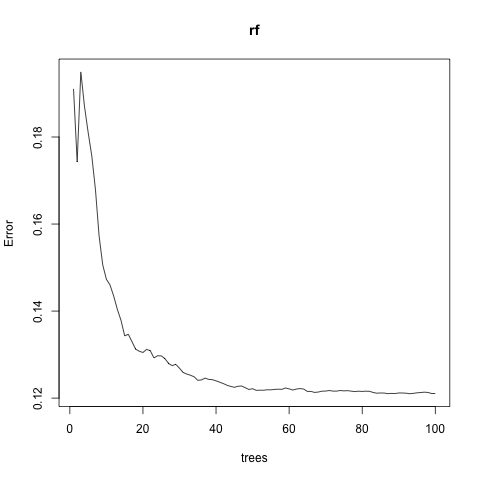
\includegraphics[width=0.5\textwidth]{../images/rf_treesgap_completion_white_black.png}
\caption{\label{fig: WBRFerror} We see that increasing the number of trees is unlikely to produce better results.}
\end{figure}

In this situation, we are not attempting to build a predictive model. We are focused on identifying interesting relationships. Still, our models performed fairly poorly in terms of percent variance explained, so we should take these results with a grain of salt.

\begin{figure}[H]
\centering
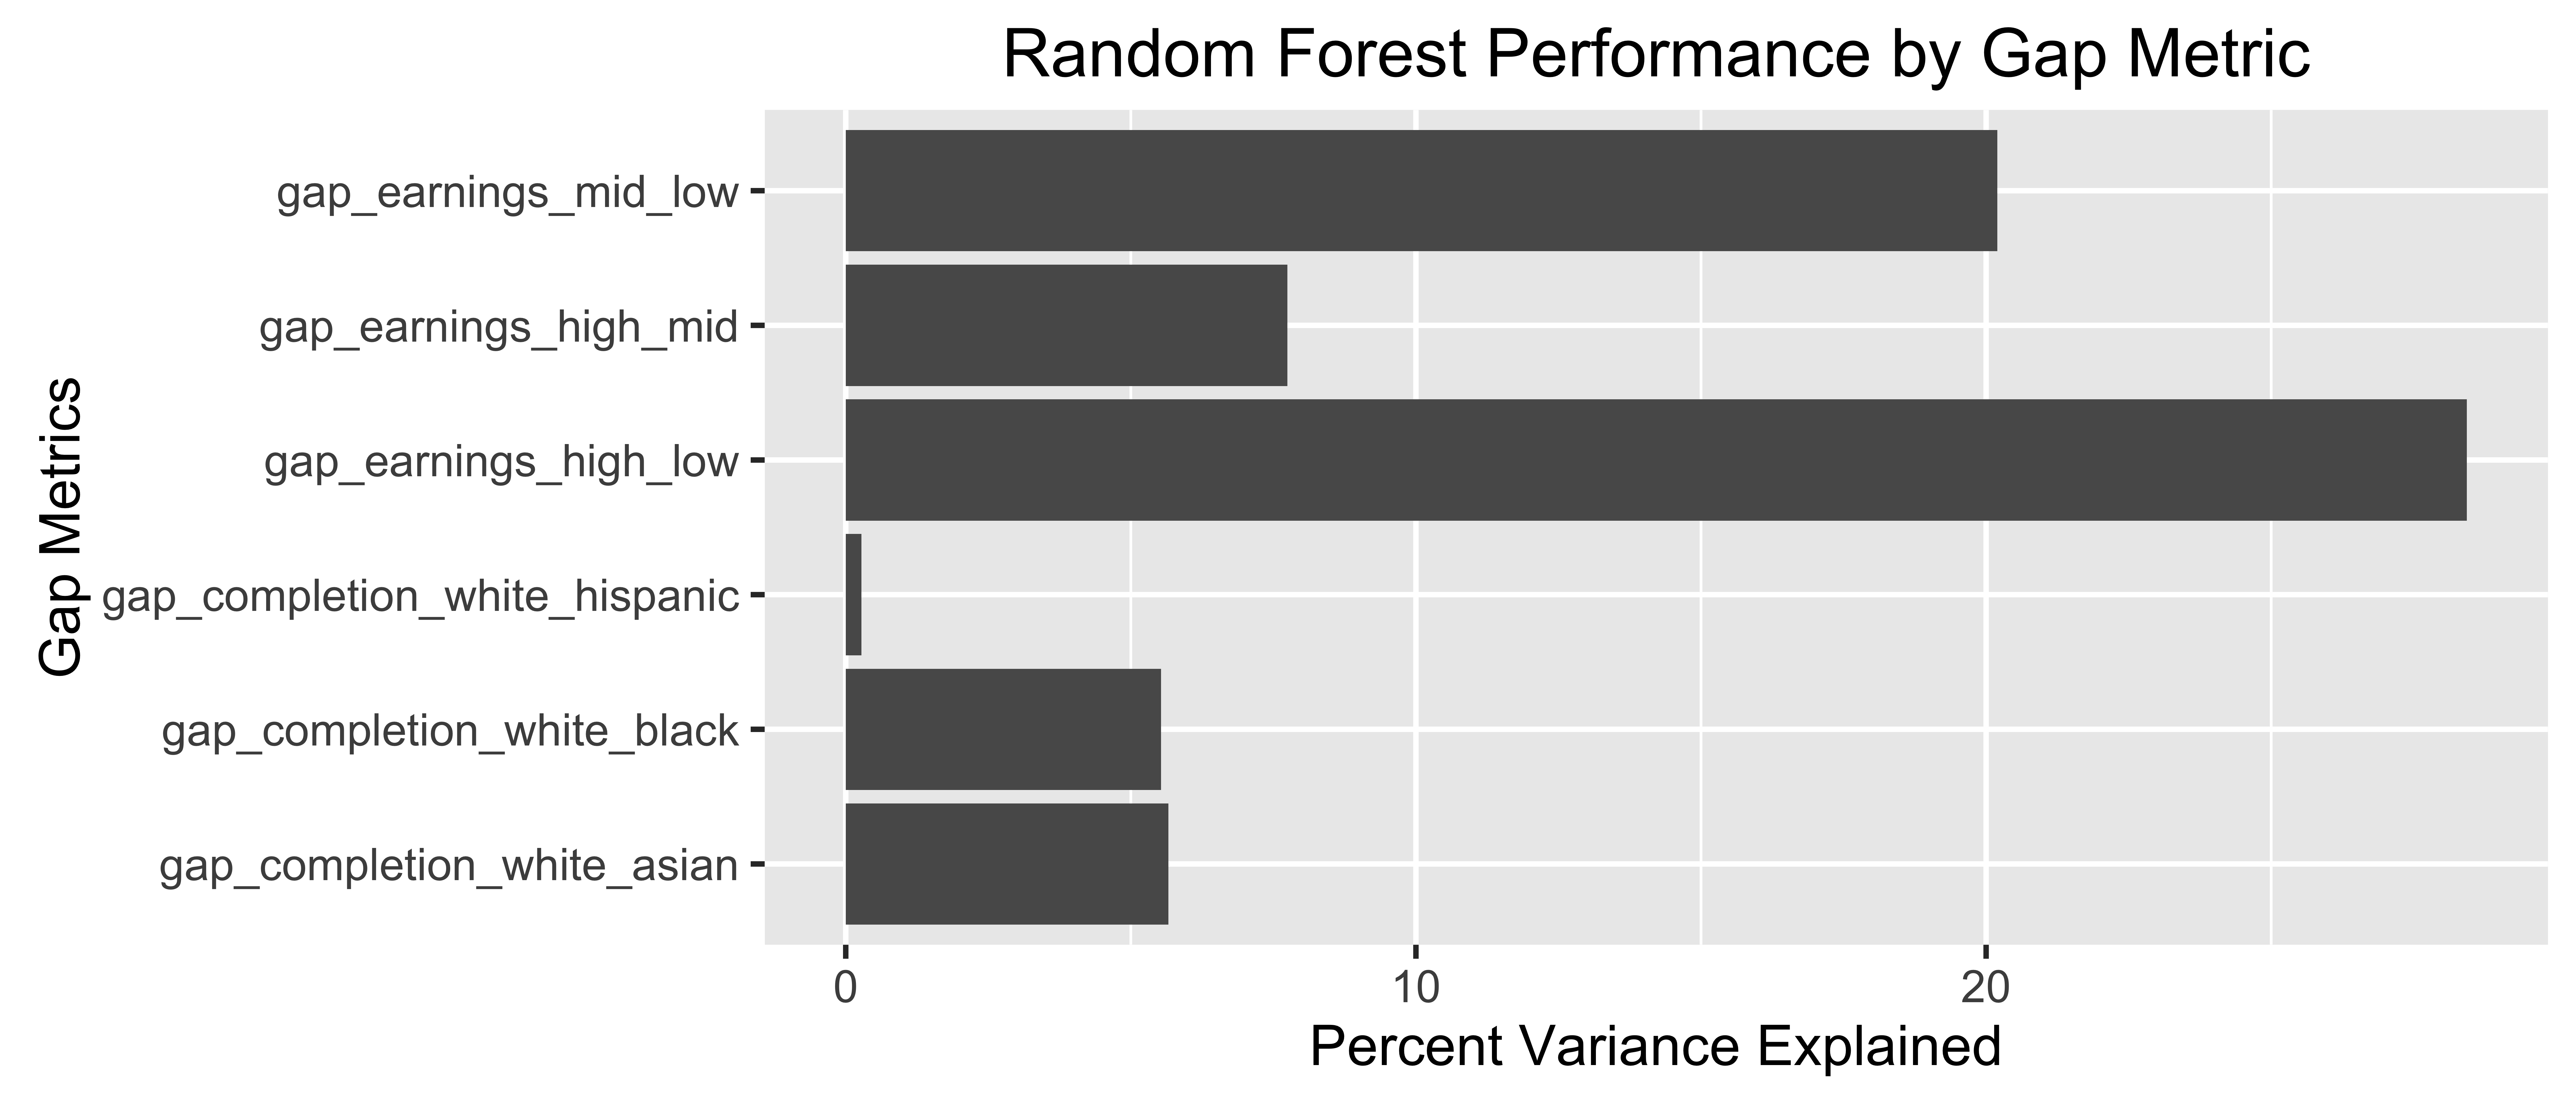
\includegraphics[width=0.5\textwidth]{../images/rf_performance.png}
\caption{\label{fig: CompletionRatesCohorts} Most of our Random Forests performed extremely poorly. The best model was that which explained the variance between High and Low Income terciles. Interestingly, this recalls that the most visually noticeable trend in EDA was between these groups.}
\end{figure}

The reason we chose random forest was that this model provides a heuristic for variable importance. This statistic is the result of caculating the average increase in node purity associated with each variable over all one hundred trees. This metric is difficult to understand without some conception of how a decision tree is constructed, but an abstract explanation is that the statistic indicates how much more accurate a tree is in predicting the target when given the variable. Therefore, a comparison of node purity increase across the variables for the separate models can provide some insight for our purposes.

Because the spread of the completion rate gaps was much larger than the spread of earning gaps, we consider these types separately.


\begin{figure}[H]
\centering
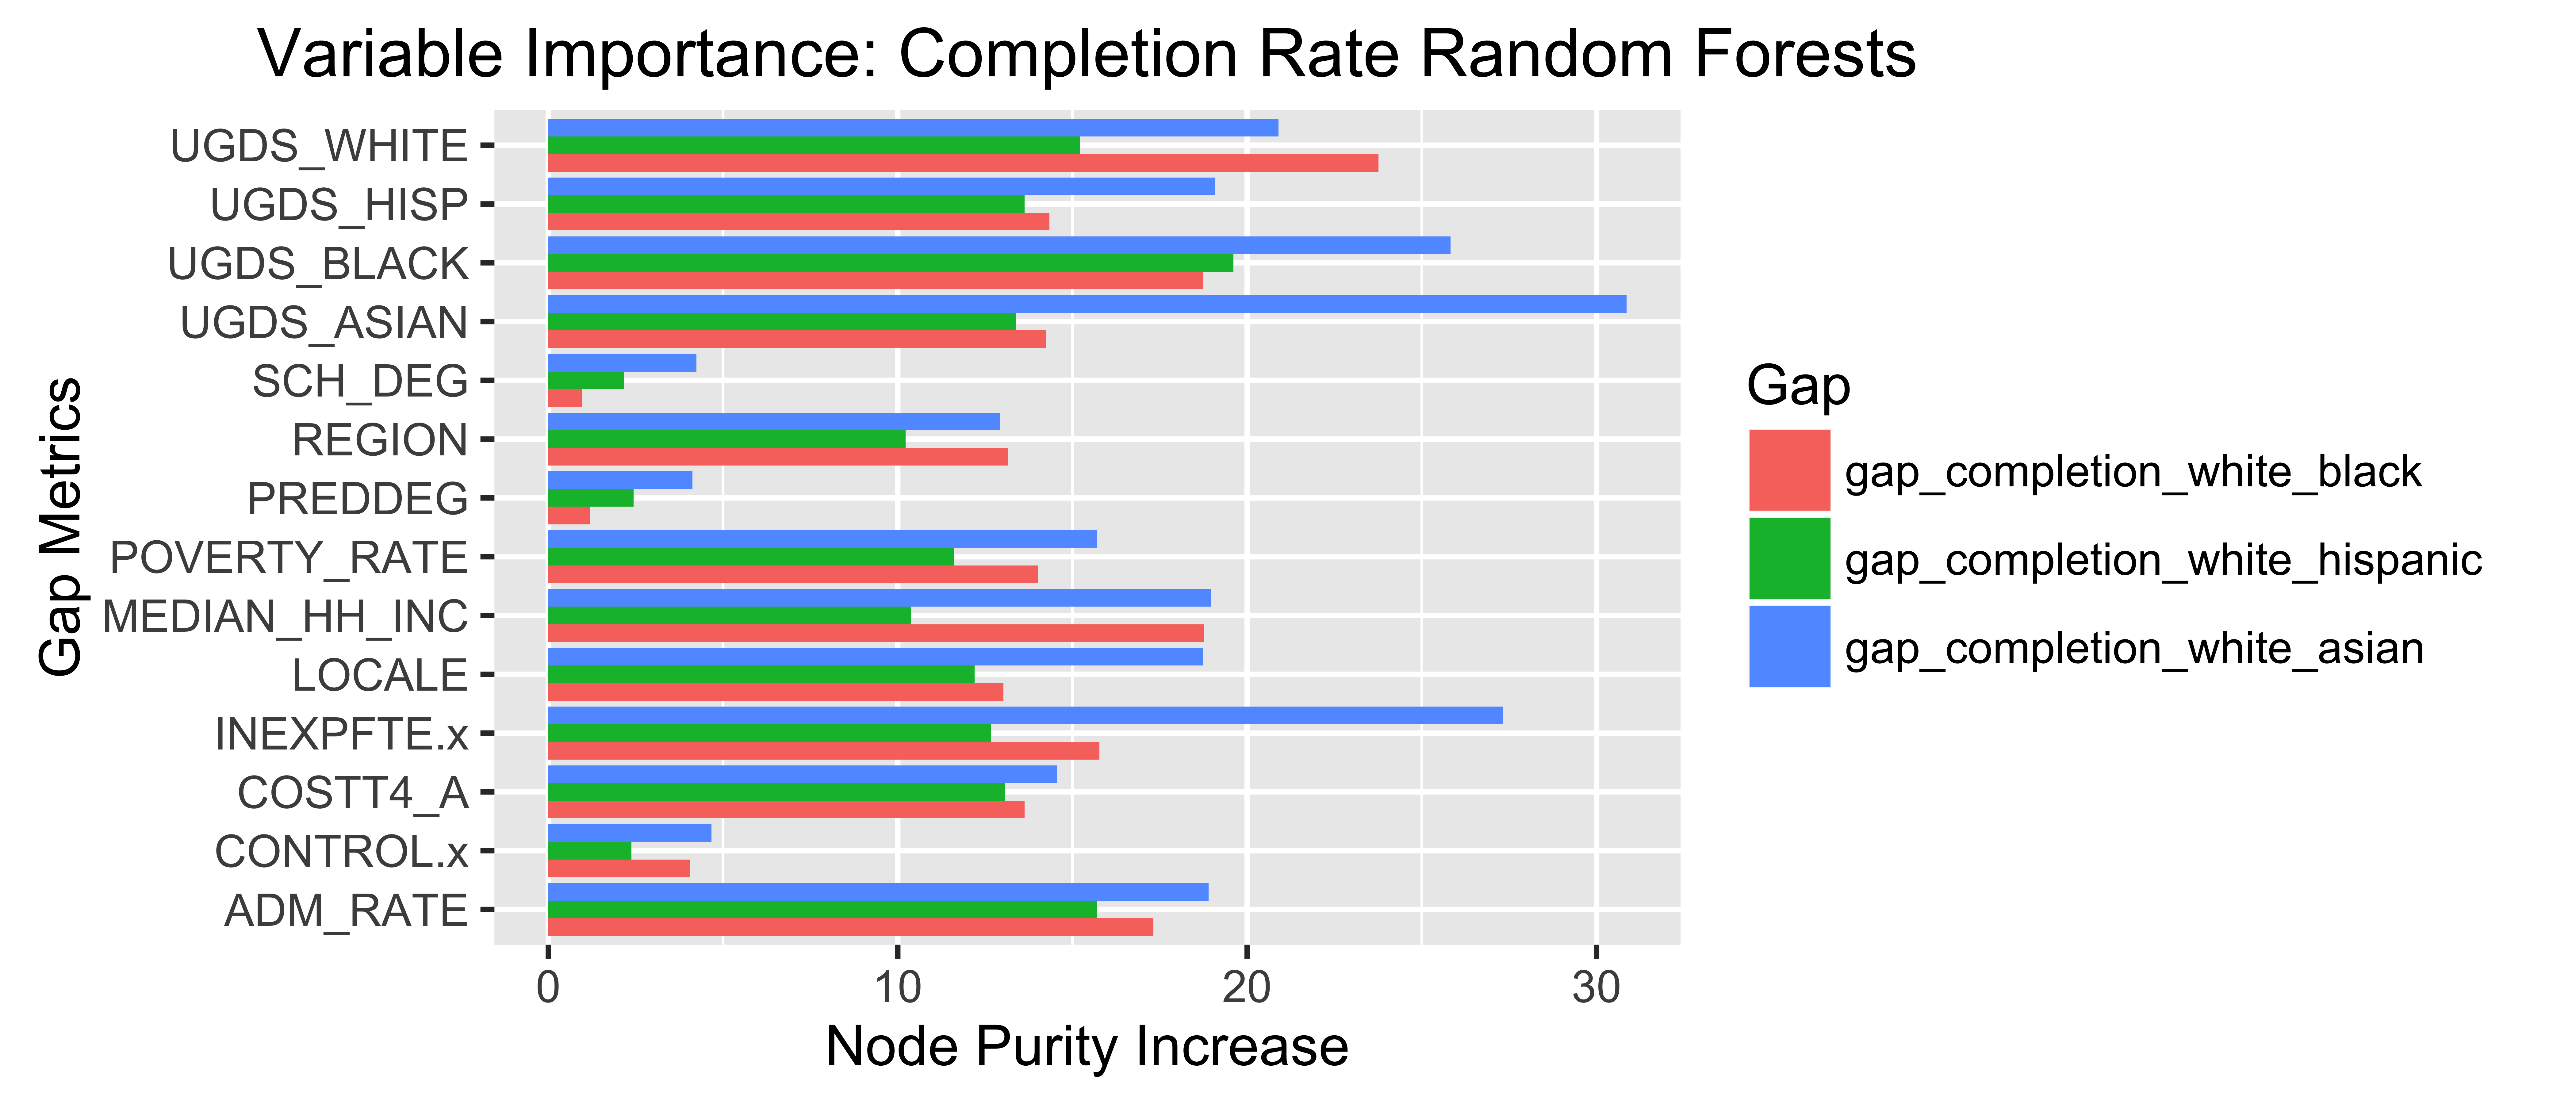
\includegraphics[width=0.5\textwidth]{../images/rf_importance_completion.png}
\caption{\label{fig: CompletionRatesCohorts} The most notable takeaway is that INEXPFTE is in fact one of the most important predictors, especially for the white Asian gap. Recall that this model performed the best of the completion rate models. Another noticeable trend is that the proportion of the student body which is Asian is a strong predictor for the white Asian completion gap. We also see a similar trend with the UGDSBlack for the white black completion gap. Generally, the diversity of the student body seems to be fairly relevant.}
\end{figure}



\begin{figure}[H]
\centering
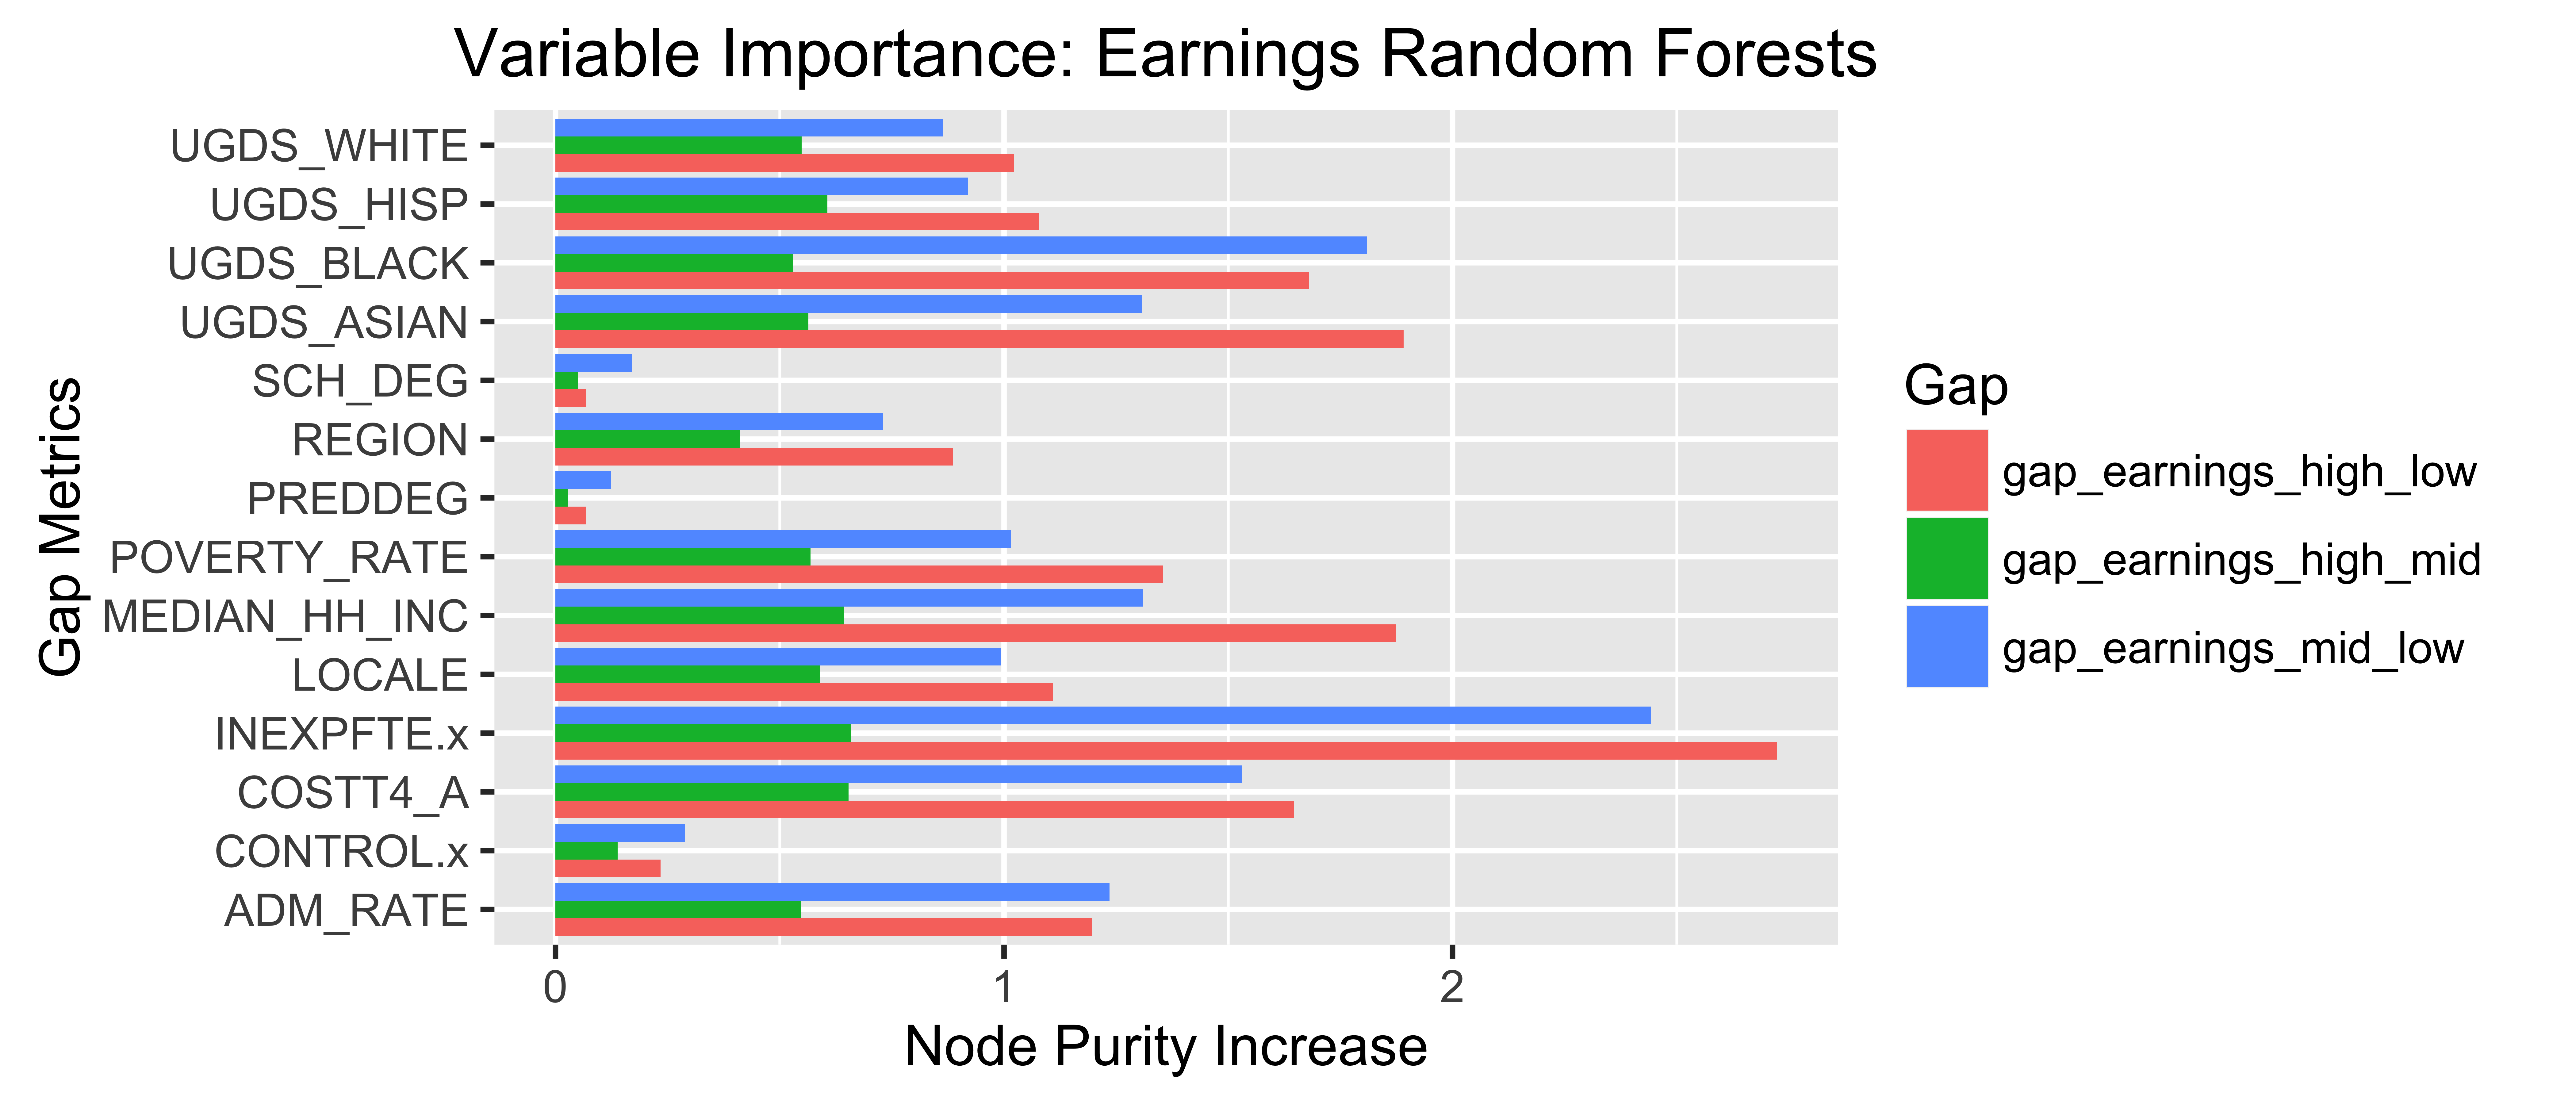
\includegraphics[width=0.5\textwidth]{../images/rf_importance_earnings.png}
\caption{\label{fig: EarningsRFImportance} Here again, we see that INEXPFTE is the strongest variable for the best performing model, high low. We also notice that Median Household Income and Cost to Attend are stronger in these models, which intutitively makes sense given that we are comparing groups according to parent income. Interestingly, UGDSBLACK and UGDSASIAN are fairly important as well.}
\end{figure}

Relating these results to our previous analysis, we find that overall, Expenditures per Student seems to have a stronger relationship with outcome gaps than most other variables, while CONTROL is actually consistently one of the weakest variables. 


\end{document}
